\section{Methods}
\subsection{Metrics}
For each graph, the x axis signifies number of epochs of training, and the y axis signifies accuracy. Accuracy is calculated after the synchronisation step, by checking the number of correct predictions on an unseen test set.

\subsection{Data Collection}
For each set of parameters to the algorithm, training was repeated 5 times, and the accuracies for each node from every run were recorded. For each timestep, the accuracy was taken to be the median accuracy between all nodes across all runs at that timestep. This helped to reduce noise in the performance metrics.

\subsection{Node Counts}
All experiments were run with 10 nodes, excluding the server when using federated learning. This number was chosen as it was the highest node count that could be achieved without the training machine's resources being exhausted and crashing.

\subsection{Choosing Parameters}
The proposed algorithm has three adjustable parameters, each of which can take one of many different values, resulting in a very large search space for optimal parameters. Therefore, rather than changing one parameter at a time and comparing results, it was decided to simulate all possible arrangements of parameters and then apply a grid search to determine the best parameter sets. Conclusions could then be made by analysing the optimal parameter sets and looking for patterns.

However, a scalar metric for performance must be established for grid search to be performed. As each set of parameters produces a graph, not a scalar, a metric function was applied to each graph that would reflect a real-world application. These metrics are discussed in further detail below.

\section{Experiments}
\subsection{Optimising for Peak Accuracy}
Details:
\begin{itemize}
	\item Sorted by peak accuracy
	\item To get the absolutely highest performing models
\end{itemize}


\begin{figure}
	\centering
	\subfloat[\centering label 1]{{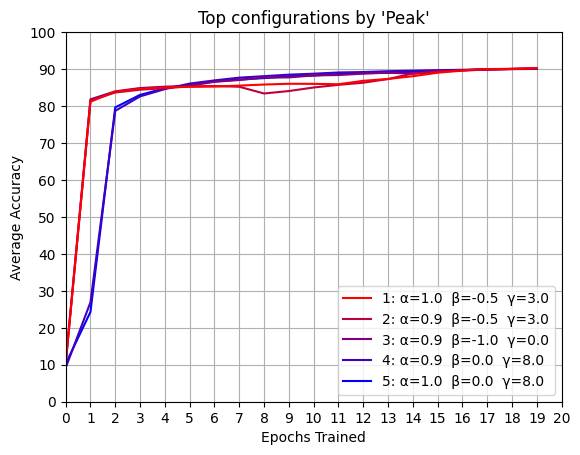
\includegraphics[width=0.75\textwidth]{ex_peak_a} }}%
	\qquad
	\subfloat[\centering label 2]{{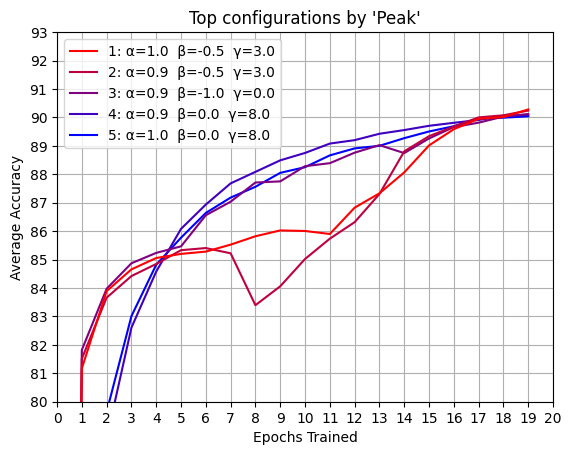
\includegraphics[width=0.75\textwidth]{ex_peak_b} }}%
	\caption{2 Figures side by side}%
	\label{fig:ex_peak}%
\end{figure}

Analysis:
\begin{itemize}
	\item Not stable
	\item Slower training at the start
	\item high alpha, negative beta, low gamma gives the top 3
	\item the other two have high alpha, 0 beta, high gamma
	\item not a good metric
\end{itemize}

\subsection{Optimising for Graph Area}
Details:
\begin{itemize}
	\item Sorted by area under the graph
	\item To get the fast training and continuously high accuracy
\end{itemize}

\begin{figure}
	\centering
	\subfloat[\centering label 1]{{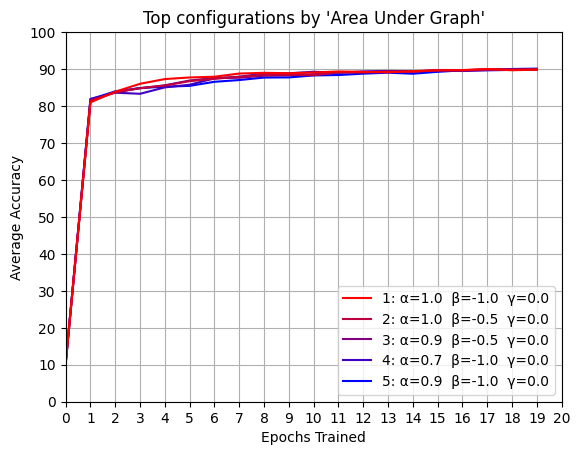
\includegraphics[width=0.75\textwidth]{ex_aug_a} }}%
	\qquad
	\subfloat[\centering label 2]{{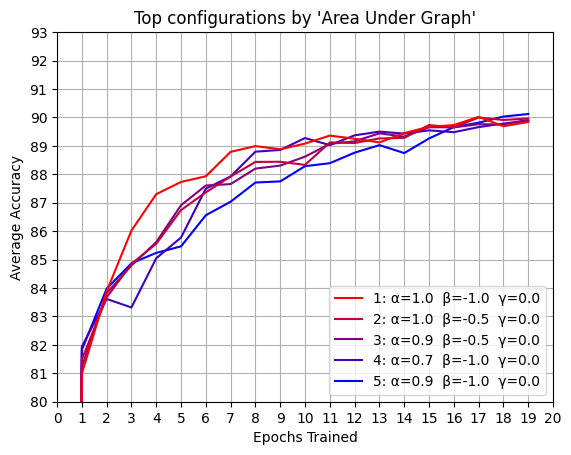
\includegraphics[width=0.75\textwidth]{ex_aug_b} }}%
	\caption{2 Figures side by side}%
	\label{fig:ex_aug}%
\end{figure}

Analysis:
\begin{itemize}
	\item Noisy but stable overall
	\item Fast start to training
	\item high alpha, between -1 and -0.5 beta, 0 gamma
	\item good if you want fast training, but not good if stability is required
\end{itemize}

\subsection{Optimising for Stability}
Details:
\begin{itemize}
	\item Sorted by stability (total amount of downwards moment)
	\item To get stable and non-noisy training
\end{itemize}

\begin{figure}
	\centering
	\subfloat[\centering label 1]{{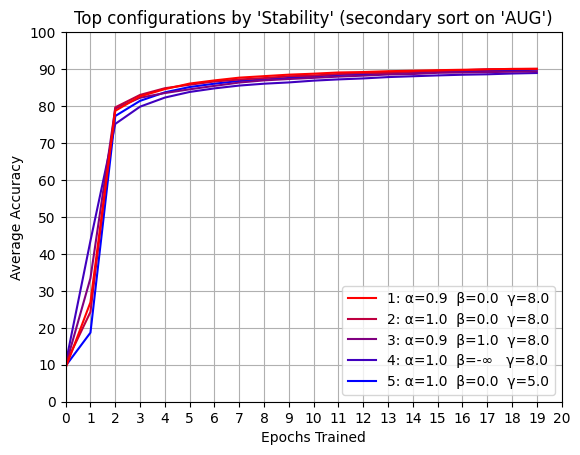
\includegraphics[width=0.75\textwidth]{ex_stab_a} }}%
	\qquad
	\subfloat[\centering label 2]{{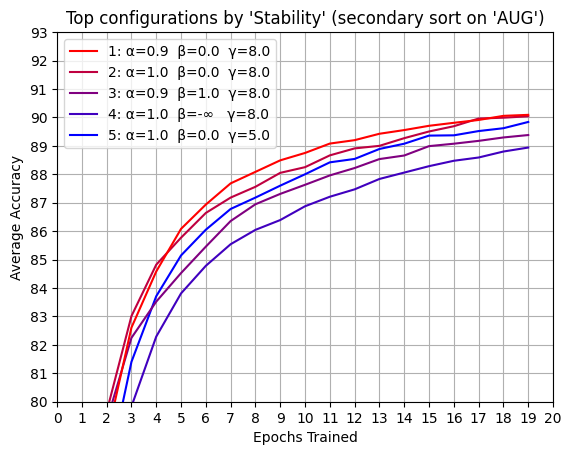
\includegraphics[width=0.75\textwidth]{ex_stab_b} }}%
	\caption{2 Figures side by side}%
	\label{fig:ex_stab}%
\end{figure}

Analysis:
\begin{itemize}
	\item Smooth training
	\item No dips - reliable
	\item high alpha, beta doesnt matter, high gamma
	\item good if you want fast training, but not good if stability is required
\end{itemize}

\subsection{Summary of Different Parameters}
What do each of the parameters do?

\subsection{Comparison with Federated Learning}
In this experiment, the top parameter sets from each category are shown next to federated learning.